\documentclass[xetex,18pt,aspectratio=43]{beamer}

\usepackage{caption}
\usepackage[percent]{overpic}
\usepackage{xecyr}
\usepackage{xunicode}
\usepackage[absolute,overlay]{textpos}
\usepackage{fontspec}
\usepackage{calc}
\usepackage{multicol}
\usepackage{hyperref}
\usepackage{setspace}
\usepackage{tikz}
%\usepackage{coloremoji}
\usepackage{csquotes}
\usepackage[export]{adjustbox}
\usepackage[normalem]{ulem}
%\usepackage{cancel}
%\usepackage[texcoord,grid,gridunit=mm,gridcolor=red!10,subgridcolor=green!10]{eso-pic}
\defaultfontfeatures{Ligatures=TeX}
\setmainfont{Trebuchet MS}
\usepackage{polyglossia}
\setdefaultlanguage[spelling=modern]{russian}
\newfontfamily{\cyrillicfont}{Trebuchet MS}
\newfontfamily{\cyrillicfontsf}{Trebuchet MS}
\newfontfamily{\cyrillicfonttt}{Trebuchet MS}
\newfontface\lserif{Microsoft Sans Serif}

\newcommand\Bigfont{\fontsize{20}{20}\selectfont}
\newcommand\Authorfont{\fontsize{17}{17}\selectfont}
\newcommand\Orgfont{\fontsize{13}{13}\selectfont}

\definecolor{cadmiumgreen}{rgb}{0.0, 0.42, 0.24}
\definecolor{darkpastelgreen}{rgb}{0.01, 0.75, 0.24}
\definecolor{darkorange}{rgb}{1.0, 0.55, 0.0}
\definecolor{darkorchid}{rgb}{0.6, 0.2, 0.8}
\definecolor{darkpink}{rgb}{0.91, 0.33, 0.5}
\definecolor{bgcolor}{RGB}{23, 33, 43}
\definecolor{fgcolor}{RGB}{127, 145, 164}
\definecolor{lightfgcolor}{RGB}{187, 205, 224}
\definecolor{titlecolor}{RGB}{130, 179, 219}
\definecolor{linkcolor}{RGB}{65, 120, 253}

\mode<presentation>
{
  %\usetheme{Boadilla}      % or try Darmstadt, Madrid, Warsaw, ...
  \usecolortheme{default} % or try albatross, beaver, crane, ...
  %\usefonttheme{default}  % or try serif, structurebold, ...
  \setbeamertemplate{navigation symbols}{}
  \setbeamertemplate{caption}[numbered]
  \setbeamertemplate{itemize items}[circle]
  \setbeamerfont{title}{series=\bfseries,parent=structure}
  \setbeamerfont{frametitle}{size=\huge}
} 

\makeatother
\setbeamertemplate{footline}
{
  \leavevmode%
  \hbox{%
  \begin{beamercolorbox}[wd=.35\paperwidth,ht=2.5ex,dp=1ex,center]{author in head/foot}%
    \usebeamerfont{author in head/foot}\insertshortauthor
  \end{beamercolorbox}%
  \begin{beamercolorbox}[wd=.65\paperwidth,ht=2.5ex,dp=1ex,center]{title in head/foot}%
    \usebeamerfont{title in head/foot}\insertshorttitle\hfill
    \insertframenumber{} / \inserttotalframenumber\hspace*{-8ex}
  \end{beamercolorbox}}%
  \vskip0pt%
}
\makeatletter

\title[Базы данных в Kubernetes]{}
\author[Александр Чистяков, vdsina.ru]{}
\date{}

\begin{document}

{ % all template changes are local to this group.
    \setbeamertemplate{navigation symbols}{}
    %\setbeamertemplate{background}[grid][step=10]
    \setbeamertemplate{background}{
\includegraphics[width=\paperwidth,height=\paperheight,keepaspectratio]{img/firstslide.png}}
    \setbeamercolor{background canvas}{bg=bgcolor}
    \setbeamercolor{item}{fg=fgcolor}
    \setbeamercolor{normal text}{fg=fgcolor}
    \usebeamercolor[fg]{normal text}
    \begin{frame}[plain]
      \setstretch{1.2}
      \begin{textblock*}{\framewidth}(0.95cm,3.0cm) % {block width} (coords)
        \Bigfont
          \begin{center}
          Базы данных в Kubernetes
          \end{center}
      \end{textblock*}
      \begin{textblock*}{\framewidth}(0.95cm,5.8cm) % {block width} (coords)
        \Authorfont
          \begin{center}
          Александр Чистяков
          \end{center}
      \end{textblock*}
      \begin{textblock*}{\framewidth}(0.95cm,6.9cm) % {block width} (coords)
        \Orgfont
          \begin{center}
          \href{https://vdsina.ru}{\color{linkcolor}vdsina.ru}, евангелист
          \end{center}
      \end{textblock*}
     \end{frame}
}


\begin{Large}

\setbeamercolor{background canvas}{bg=bgcolor}
\setbeamercolor{item}{fg=fgcolor}
\setbeamercolor{normal text}{fg=fgcolor}
\setbeamercolor{author in head/foot}{fg=lightfgcolor}
\setbeamercolor{title in head/foot}{fg=lightfgcolor}
\setbeamercolor{frametitle}{fg=titlecolor}
\usebeamercolor[fg]{normal text}

\begin{frame}{\ \ \ Очень краткое содержание}
\setstretch{1.2}
\begin{textblock*}{\framewidth+0.9cm}(0.5cm,1.5cm)
\begin{itemize}
  \item Отказ от ответственности
  \item Зачем?
  \item План развертывания
  \item Примеры использования
  \item Как мы ходили в горы и упали (*)
\end{itemize}
\end{textblock*}
\end{frame}

\begin{frame}{\ \ \ Отказ от ответственности}
\setstretch{1.2}
\begin{textblock*}{\framewidth+0.9cm}(0.5cm,1.5cm)
\begin{itemize}
  \item Я не психотерапевт и не знаю, можно ли вам
\end{itemize}
\begin{minipage}{\textwidth}
  \centering
  
\includegraphics[height=6.0cm]{img/dont}
\end{minipage}
\end{textblock*}
\end{frame}

\begin{frame}{\ \ \ Зачем?}
\setstretch{1.2}
\begin{textblock*}{\framewidth+0.9cm}(0.5cm,1.5cm)
\begin{itemize}
  \item Унификация инфраструктуры (WAT?)
\end{itemize}
\end{textblock*}
\end{frame}

\begin{frame}{\ \ \ Зачем?}
\setstretch{1.2}
\begin{textblock*}{\framewidth+0.9cm}(0.5cm,1.5cm)
\begin{itemize}
  \item Унификация инфраструктуры
  \item (Развертывание, мониторинг, обсервабилити, управление жизненным циклом)
\end{itemize}
\end{textblock*}
\end{frame}

\begin{frame}{\ \ \ Зачем?}
\setstretch{1.2}
\begin{textblock*}{\framewidth+0.9cm}(0.5cm,1.5cm)
\begin{itemize}
  \item Унификация инфраструктуры
  \item (Развертывание, мониторинг, обсервабилити, управление жизненным циклом)
  \item Антикитерский механизм
\end{itemize}
\end{textblock*}
\end{frame}

\begin{frame}{\ \ \ Зачем?}
\setstretch{1.2}
\begin{textblock*}{\framewidth+0.9cm}(0.5cm,1.5cm)
\begin{itemize}
  \item Унификация инфраструктуры
  \item (Развертывание, мониторинг, обсервабилити, управление жизненным циклом)
  \item Антикитерский механизм
  \item (Обсудим это позже)
\end{itemize}
\begin{minipage}{\textwidth}
  \centering
  
\includegraphics[height=3.5cm]{img/dont2}
\end{minipage}
\end{textblock*}
\end{frame}

\begin{frame}{\ \ \ План развертывания - история}
\setstretch{1.2}
\begin{textblock*}{\framewidth+0.9cm}(0.5cm,1.5cm)
\begin{itemize}
  \item Я начал эксперименты в июне 2018-го
\end{itemize}
\end{textblock*}
\end{frame}

\begin{frame}{\ \ \ План развертывания - история}
\setstretch{1.2}
\begin{textblock*}{\framewidth+0.9cm}(0.5cm,1.5cm)
\begin{itemize}
  \item Я начал эксперименты в июне 2018-го
  \item В то время логичным выбором был Helm
\end{itemize}
\end{textblock*}
\end{frame}

\begin{frame}{\ \ \ План развертывания - история}
\setstretch{1.2}
\begin{textblock*}{\framewidth+0.9cm}(0.5cm,1.5cm)
\begin{itemize}
  \item Я начал эксперименты в июне 2018-го
  \item В то время логичным выбором был Helm
\end{itemize}
\begin{minipage}{\textwidth}
  \centering
  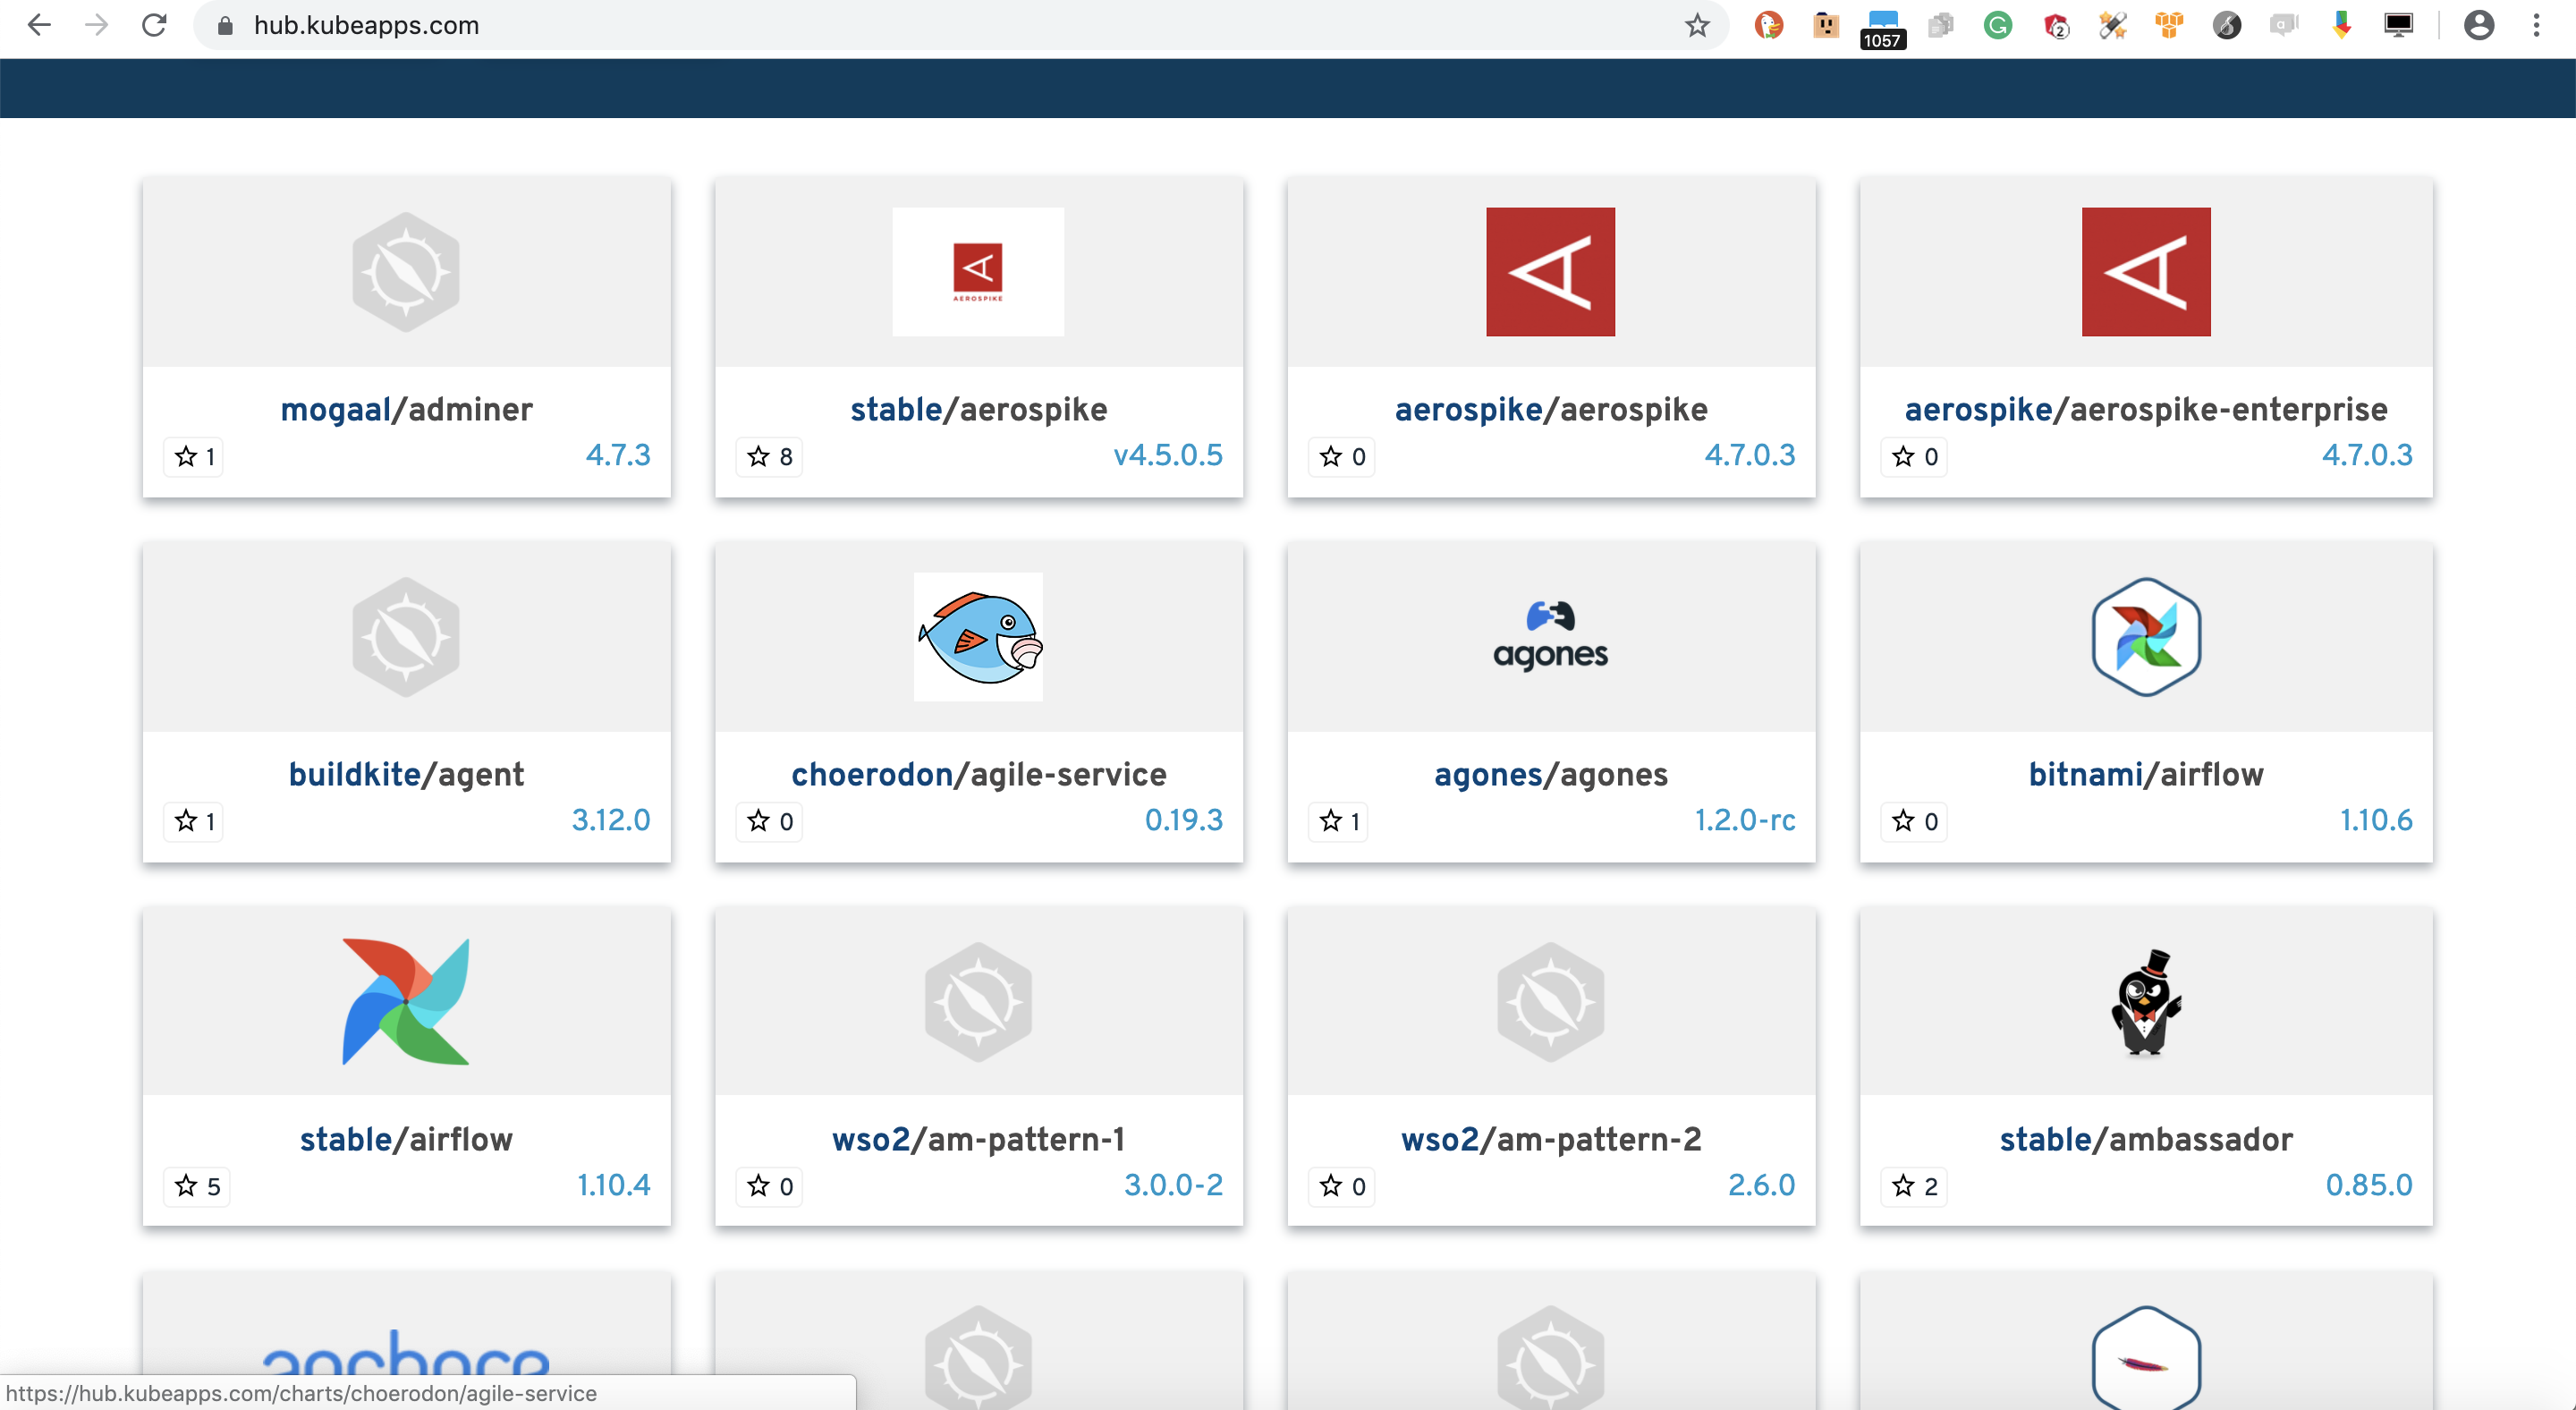
\includegraphics[height=6.0cm]{img/kubeapps}
\end{minipage}
\end{textblock*}
\end{frame}

\begin{frame}{\ \ \ План развертывания - Helm}
\setstretch{1.2}
\begin{textblock*}{\framewidth+0.9cm}(0.5cm,1.5cm)
\begin{itemize}
  \item Найти нужный chart
\end{itemize}
\end{textblock*}
\end{frame}

\begin{frame}{\ \ \ План развертывания - Helm}
\setstretch{1.2}
\begin{textblock*}{\framewidth+0.9cm}(0.5cm,1.5cm)
\begin{itemize}
  \item Найти нужный chart
  \item Переопределить нужные values
\end{itemize}
\end{textblock*}
\end{frame}

\begin{frame}{\ \ \ План развертывания - Helm}
\setstretch{1.2}
\begin{textblock*}{\framewidth+0.9cm}(0.5cm,1.5cm)
\begin{itemize}
  \item Найти нужный chart
  \item Переопределить нужные values
  \item Применить
\end{itemize}
\end{textblock*}
\end{frame}

\begin{frame}{\ \ \ План развертывания - Helm}
\setstretch{1.2}
\begin{textblock*}{\framewidth+0.9cm}(0.5cm,1.5cm)
\begin{itemize}
  \item Найти нужный chart
  \item Переопределить нужные values
  \item Применить
  \item Еще надо где-то хранить состояние (данные)
\end{itemize}
\end{textblock*}
\end{frame}

\begin{frame}{\ \ \ Где хранить данные?}
\setstretch{1.2}
\begin{textblock*}{\framewidth+0.9cm}(0.5cm,1.5cm)
\begin{itemize}
  \item Если вы уже в облаке - храните в облаке
\end{itemize}
\end{textblock*}
\end{frame}

\begin{frame}{\ \ \ Где хранить данные?}
\setstretch{1.2}
\begin{textblock*}{\framewidth+0.9cm}(0.5cm,1.5cm)
\begin{itemize}
  \item Если вы уже в облаке - храните в облаке
  \item (AWS, Google Cloud)
\end{itemize}
\end{textblock*}
\end{frame}

\begin{frame}{\ \ \ Где хранить данные?}
\setstretch{1.2}
\begin{textblock*}{\framewidth+0.9cm}(0.5cm,1.5cm)
\begin{itemize}
  \item Если вы уже в облаке - храните в облаке
  \item (AWS, Google Cloud)
  \item Если on-prem - храните на локальных дисках
\end{itemize}
\end{textblock*}
\end{frame}

\begin{frame}{\ \ \ Плюсы локальных дисков}
\setstretch{1.2}
\begin{textblock*}{\framewidth+0.9cm}(0.5cm,1.5cm)
\begin{itemize}
  \item Это просто
\end{itemize}
\end{textblock*}
\end{frame}

\begin{frame}{\ \ \ Плюсы локальных дисков}
\setstretch{1.2}
\begin{textblock*}{\framewidth+0.9cm}(0.5cm,1.5cm)
\begin{itemize}
  \item Это просто
  \item Не требует создания распределенного хранилища
\end{itemize}
\end{textblock*}
\end{frame}

\begin{frame}{\ \ \ Плюсы локальных дисков}
\setstretch{1.2}
\begin{textblock*}{\framewidth+0.9cm}(0.5cm,1.5cm)
\begin{itemize}
  \item Это просто
  \item Не требует создания распределенного хранилища
  \item Не требует дополнительного обслуживания
\end{itemize}
\end{textblock*}
\end{frame}

\begin{frame}{\ \ \ Минусы локальных дисков}
\setstretch{1.2}
\begin{textblock*}{\framewidth+0.9cm}(0.5cm,1.5cm)
\begin{itemize}
  \item Отказоустойчивость и масштабирование делаются извне
\end{itemize}
\end{textblock*}
\end{frame}

\begin{frame}{\ \ \ Минусы локальных дисков}
\setstretch{1.2}
\begin{textblock*}{\framewidth+0.9cm}(0.5cm,1.5cm)
\begin{itemize}
  \item Отказоустойчивость и масштабирование делаются извне
  \item Данные хранятся на тех же мощностях, что и кластер
\end{itemize}
\end{textblock*}
\end{frame}

\begin{frame}{\ \ \ Минусы локальных дисков}
\setstretch{1.2}
\begin{textblock*}{\framewidth+0.9cm}(0.5cm,1.5cm)
\begin{itemize}
  \item Отказоустойчивость и масштабирование делаются извне
  \item Данные хранятся на тех же мощностях, что и кластер
  \item В случае потери метаинформации найти, где было что, очень сложно
\end{itemize}
\end{textblock*}
\end{frame}

\begin{frame}{\ \ \ Другие варианты on-prem}
\setstretch{1.2}
\begin{textblock*}{\framewidth+0.9cm}(0.5cm,1.5cm)
\begin{itemize}
  \item GlusterFS
\end{itemize}
\end{textblock*}
\end{frame}

\begin{frame}{\ \ \ Другие варианты on-prem}
\setstretch{1.2}
\begin{textblock*}{\framewidth+0.9cm}(0.5cm,1.5cm)
\begin{itemize}
  \item GlusterFS
  \item Ceph
\end{itemize}
\end{textblock*}
\end{frame}

\begin{frame}{\ \ \ Другие варианты on-prem}
\setstretch{1.2}
\begin{textblock*}{\framewidth+0.9cm}(0.5cm,1.5cm)
\begin{itemize}
  \item GlusterFS
  \item Ceph
  \item \href{https://rook.io}{\color{linkcolor}{rook.io}} (Ceph в
    том же K8s кластере)
\end{itemize}
\end{textblock*}
\end{frame}

\begin{frame}{\ \ \ Другие варианты on-prem}
\setstretch{1.2}
\begin{textblock*}{\framewidth+0.9cm}(0.5cm,1.5cm)
\begin{itemize}
  \item GlusterFS
  \item Ceph
  \item \href{https://rook.io}{\color{linkcolor}{rook.io}} (Ceph в
    том же K8s кластере)
  \item (Последнее я сам не пробовал и советовать не могу)
\end{itemize}
\end{textblock*}
\end{frame}

\begin{frame}{\ \ \ Другие варианты on-prem}
\setstretch{1.2}
\begin{textblock*}{\framewidth+0.9cm}(0.5cm,1.5cm)
\begin{itemize}
  \item GlusterFS
  \item Ceph
  \item \href{https://rook.io}{\color{linkcolor}{rook.io}} (Ceph в
    том же K8s кластере)
  \item (Последнее я сам не пробовал и советовать не могу)
  \item \href{https://rook.io}{\color{linkcolor}{rook.io}} использует Флант
\end{itemize}
\end{textblock*}
\end{frame}

\begin{frame}{\ \ \ Helm - Stolon}
\setstretch{1.2}
\begin{textblock*}{\framewidth+0.9cm}(0.5cm,1.5cm)
\begin{itemize}
  \item Stolon - как Patroni, но на Go
\end{itemize}
\end{textblock*}
\end{frame}

\begin{frame}{\ \ \ Helm - Stolon}
\setstretch{1.2}
\begin{textblock*}{\framewidth+0.9cm}(0.5cm,1.5cm)
\begin{itemize}
  \item Stolon - как Patroni, но на Go
  \item \href{https://github.com/alexclear/k8s-stolon-lab}{\color{linkcolor}{github.com/alexclear/k8s-stolon-lab}}
\end{itemize}
\end{textblock*}
\end{frame}

\begin{frame}{\ \ \ Helm - Patroni}
\setstretch{1.2}
\begin{textblock*}{\framewidth+0.9cm}(0.5cm,1.5cm)
\begin{itemize}
  \item Patroni - как Stolon, но на Python
\end{itemize}
\end{textblock*}
\end{frame}

\begin{frame}{\ \ \ Helm - Patroni}
\setstretch{1.2}
\begin{textblock*}{\framewidth+0.9cm}(0.5cm,1.5cm)
\begin{itemize}
  \item Patroni - как Stolon, но на Python
  \item \href{https://github.com/alexclear/k8s-patroni-lab}{\color{linkcolor}{github.com/alexclear/k8s-patroni-lab}}
\end{itemize}
\end{textblock*}
\end{frame}

\begin{frame}{\ \ \ Helm - XtraDB}
\setstretch{1.2}
\begin{textblock*}{\framewidth+0.9cm}(0.5cm,1.5cm)
\begin{itemize}
  \item XtraDB - как Galera, но от Percona
\end{itemize}
\end{textblock*}
\end{frame}

\begin{frame}{\ \ \ Helm - XtraDB}
\setstretch{1.2}
\begin{textblock*}{\framewidth+0.9cm}(0.5cm,1.5cm)
\begin{itemize}
  \item XtraDB - как Galera, но от Percona
  \item \href{https://github.com/alexclear/k8s-percona-xtradb-cluster-lab}{\color{linkcolor}{github.com/alexclear/k8s-percona-xtradb-cluster-lab}}
\end{itemize}
\end{textblock*}
\end{frame}

\begin{frame}{\ \ \ Helm - EFK}
\setstretch{1.2}
\begin{textblock*}{\framewidth+0.9cm}(0.5cm,1.5cm)
\begin{itemize}
  \item EFK - как ELK, только без L
\end{itemize}
\end{textblock*}
\end{frame}

\begin{frame}{\ \ \ Helm - EFK}
\setstretch{1.2}
\begin{textblock*}{\framewidth+0.9cm}(0.5cm,1.5cm)
\begin{itemize}
  \item EFK - как ELK, только без L
  \item \href{https://github.com/alexclear/k8s-freehck-efk-lab}{\color{linkcolor}{github.com/alexclear/k8s-freehck-efk-lab}}
\end{itemize}
\end{textblock*}
\end{frame}

\begin{frame}{\ \ \ А что, если?}
\setstretch{1.2}
\begin{textblock*}{\framewidth+0.9cm}(0.5cm,1.5cm)
\begin{itemize}
  \item Если мы хотим делать бэкапы?
\end{itemize}
\end{textblock*}
\end{frame}

\begin{frame}{\ \ \ А что, если?}
\setstretch{1.2}
\begin{textblock*}{\framewidth+0.9cm}(0.5cm,1.5cm)
\begin{itemize}
  \item Если мы хотим делать бэкапы?
  \item Если мы хотим автоматически экспортировать дэшборд?
\end{itemize}
\end{textblock*}
\end{frame}

\begin{frame}{\ \ \ А что, если?}
\setstretch{1.2}
\begin{textblock*}{\framewidth+0.9cm}(0.5cm,1.5cm)
\begin{itemize}
  \item Если мы хотим делать бэкапы?
  \item Если мы хотим автоматически экспортировать дэшборд?
  \item Если мы хотим автоматически апргрейдить минорные версии?
\end{itemize}
\end{textblock*}
\end{frame}

\begin{frame}{\ \ \ А что, если?}
\setstretch{1.2}
\begin{textblock*}{\framewidth+0.9cm}(0.5cm,1.5cm)
\begin{itemize}
  \item Если мы хотим делать бэкапы?
  \item Если мы хотим автоматически экспортировать дэшборд?
  \item Если мы хотим автоматически апргрейдить минорные версии?
  \item Пересмотрим план развертывания
\end{itemize}
\end{textblock*}
\end{frame}

\begin{frame}{\ \ \ План развертывания - не Helm}
\setstretch{1.2}
\begin{textblock*}{\framewidth+0.9cm}(0.5cm,1.5cm)
\begin{itemize}
  \item Оператор = CRD + контроллер
\end{itemize}
\end{textblock*}
\end{frame}

\begin{frame}{\ \ \ План развертывания - не Helm}
\setstretch{1.2}
\begin{textblock*}{\framewidth+0.9cm}(0.5cm,1.5cm)
\begin{itemize}
  \item Оператор = CRD + контроллер
  \item CRD позволяет добавить в YAML что-то свое
\end{itemize}
\end{textblock*}
\end{frame}

\begin{frame}{\ \ \ План развертывания - не Helm}
\setstretch{1.2}
\begin{textblock*}{\framewidth+0.9cm}(0.5cm,1.5cm)
\begin{itemize}
  \item Оператор = CRD + контроллер
  \item CRD позволяет добавить в YAML что-то свое
  \item Контроллер управляет жизненным циклом этого чего-то
\end{itemize}
\end{textblock*}
\end{frame}

\begin{frame}{\ \ \ План развертывания - не Helm}
\setstretch{1.2}
\begin{textblock*}{\framewidth+0.9cm}(0.5cm,1.5cm)
\begin{itemize}
  \item Оператор = CRD + контроллер
  \item CRD позволяет добавить в YAML что-то свое
  \item Контроллер управляет жизненным циклом этого чего-то
  \item Контроллер - программа, обычно, на Go
\end{itemize}
\end{textblock*}
\end{frame}

\begin{frame}{\ \ \ План развертывания - не Helm}
\setstretch{1.2}
\begin{textblock*}{\framewidth+0.9cm}(0.5cm,1.5cm)
\begin{itemize}
  \item Оператор = CRD + контроллер
  \item CRD позволяет добавить в YAML что-то свое
  \item Контроллер управляет жизненным циклом этого чего-то
  \item Контроллер - программа, обычно, на Go
  \item (Работает оперейшнс инженером)
\end{itemize}
\end{textblock*}
\end{frame}

\begin{frame}{\ \ \ План развертывания - операторы}
\setstretch{1.2}
\begin{textblock*}{\framewidth+0.9cm}(0.5cm,1.5cm)
\begin{itemize}
  \item В муках найти работающий оператор
\end{itemize}
\end{textblock*}
\end{frame}

\begin{frame}{\ \ \ План развертывания - операторы}
\setstretch{1.2}
\begin{textblock*}{\framewidth+0.9cm}(0.5cm,1.5cm)
\begin{itemize}
  \item В муках найти работающий оператор
  \item Установить, используя Helm
\end{itemize}
\end{textblock*}
\end{frame}

\begin{frame}{\ \ \ План развертывания - операторы}
\setstretch{1.2}
\begin{textblock*}{\framewidth+0.9cm}(0.5cm,1.5cm)
\begin{itemize}
  \item В муках найти работающий оператор
  \item Установить, используя Helm
  \item Наслаждаться использованием CRD
\end{itemize}
\end{textblock*}
\end{frame}

\begin{frame}{\ \ \ Операторы - Cassandra}
\setstretch{1.2}
\begin{textblock*}{\framewidth+0.9cm}(0.5cm,1.5cm)
\begin{itemize}
  \item \href{https://github.com/alexclear/vagrant-k8s-freehck-cassandra-lab}{\color{linkcolor}{github.com/alexclear/vagrant-k8s-freehck-cassandra-lab}}
\end{itemize}
\end{textblock*}
\end{frame}

\begin{frame}{\ \ \ Как выбрать оператор?}
\setstretch{1.2}
\begin{textblock*}{\framewidth+0.9cm}(0.5cm,1.5cm)
\begin{itemize}
  \item Попробовать первый
\end{itemize}
\end{textblock*}
\end{frame}

\begin{frame}{\ \ \ Как выбрать оператор?}
\setstretch{1.2}
\begin{textblock*}{\framewidth+0.9cm}(0.5cm,1.5cm)
\begin{itemize}
  \item Попробовать первый
  \item Работает - не трогать
\end{itemize}
\end{textblock*}
\end{frame}

\begin{frame}{\ \ \ Как выбрать оператор?}
\setstretch{1.2}
\begin{textblock*}{\framewidth+0.9cm}(0.5cm,1.5cm)
\begin{itemize}
  \item Попробовать первый
  \item Работает - не трогать
  \item Не работает ни один - починить
\end{itemize}
\end{textblock*}
\end{frame}

\begin{frame}{\ \ \ Операторы - Redis}
\setstretch{1.2}
\begin{textblock*}{\framewidth+0.9cm}(0.5cm,1.5cm)
\begin{itemize}
  \item \href{https://github.com/alexclear/vagrant-k8s-freehck-redis-lab}{\color{linkcolor}{github.com/alexclear/vagrant-k8s-freehck-redis-lab}}
\end{itemize}
\end{textblock*}
\end{frame}

\begin{frame}{\ \ \ Операторы - PostgreSQL}
\setstretch{1.2}
\begin{textblock*}{\framewidth+0.9cm}(0.5cm,1.5cm)
\begin{itemize}
  \item \href{https://github.com/alexclear/vagrant-k8s-freehck-postgres-lab}{\color{linkcolor}{github.com/alexclear/vagrant-k8s-freehck-postgres-lab}}
\end{itemize}
\end{textblock*}
\end{frame}

\begin{frame}{\ \ \ Как выбрать оператор?}
\setstretch{1.2}
\begin{textblock*}{\framewidth+0.9cm}(0.5cm,1.5cm)
\begin{itemize}
  \item Тот, производителя которого вы знаете
\end{itemize}
\end{textblock*}
\end{frame}

\begin{frame}{\ \ \ Как выбрать оператор?}
\setstretch{1.2}
\begin{textblock*}{\framewidth+0.9cm}(0.5cm,1.5cm)
\begin{itemize}
  \item Тот, производителя которого вы знаете
  \item Тот, который проще развернуть
\end{itemize}
\end{textblock*}
\end{frame}

\begin{frame}{\ \ \ Операторы - ClickHouse}
\setstretch{1.2}
\begin{textblock*}{\framewidth+0.9cm}(0.5cm,1.5cm)
\begin{itemize}
  \item Не успел посмотреть, будет через неделю    
\end{itemize}
\end{textblock*}
\end{frame}

\begin{frame}{\ \ \ Какие еще операторы есть?}
\setstretch{1.2}
\begin{textblock*}{\framewidth+0.9cm}(0.5cm,1.5cm)
\begin{itemize}
  \item Тысячи их!
\end{itemize}
\begin{minipage}{\textwidth}
  \centering
  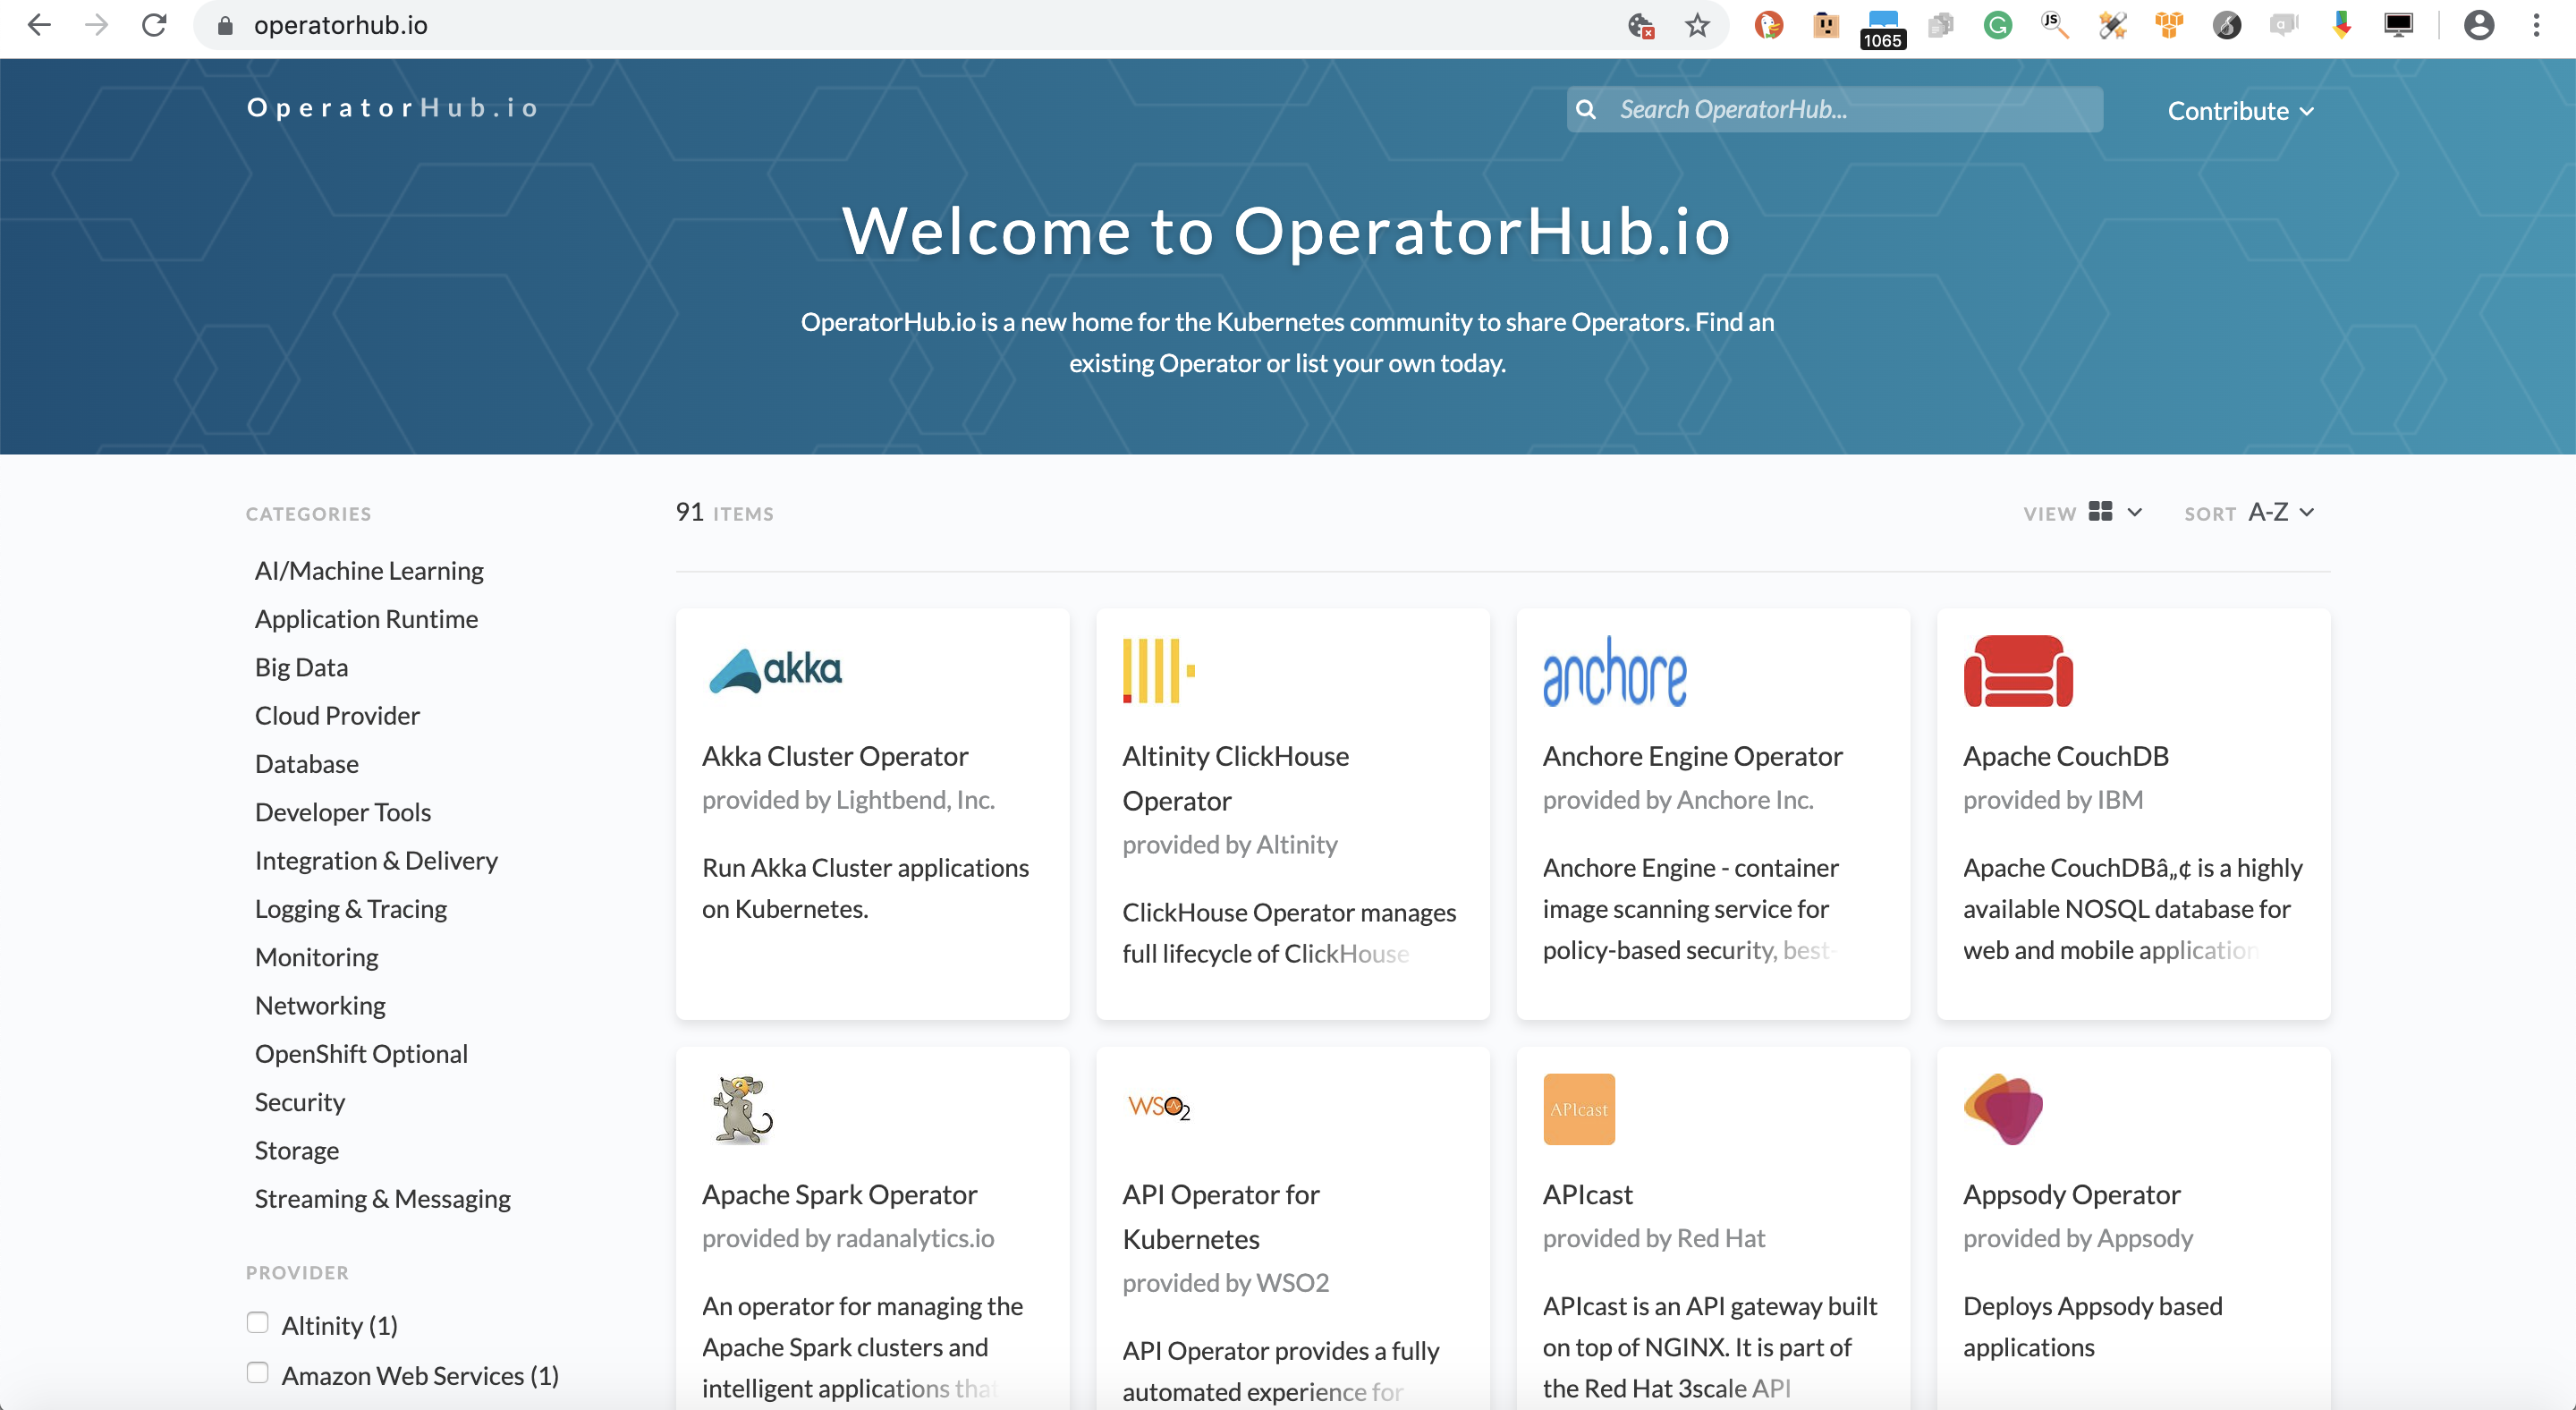
\includegraphics[height=6.0cm]{img/ophub}
\end{minipage}
\end{textblock*}
\end{frame}

\begin{frame}{\ \ \ Как мы ходили в горы}
\setstretch{1.2}
\begin{textblock*}{\framewidth+0.9cm}(0.5cm,1.5cm)
\begin{itemize}
  \item У нас был кластер K8s с хранилищем на локальных дисках
\end{itemize}
\end{textblock*}
\end{frame}

\begin{frame}{\ \ \ Как мы ходили в горы}
\setstretch{1.2}
\begin{textblock*}{\framewidth+0.9cm}(0.5cm,1.5cm)
\begin{itemize}
  \item У нас был кластер K8s с хранилищем на локальных дисках
  \item В нем EFK на каждой ноде для логов
\end{itemize}
\end{textblock*}
\end{frame}

\begin{frame}{\ \ \ Как мы ходили в горы}
\setstretch{1.2}
\begin{textblock*}{\framewidth+0.9cm}(0.5cm,1.5cm)
\begin{itemize}
  \item У нас был кластер K8s с хранилищем на локальных дисках
  \item В нем EFK на каждой ноде для логов
  \item K8s мастер был один, в виртуалке на каком-то левом хосте
\end{itemize}
\end{textblock*}
\end{frame}

\begin{frame}{\ \ \ Как мы ходили в горы}
\setstretch{1.2}
\begin{textblock*}{\framewidth+0.9cm}(0.5cm,1.5cm)
\begin{itemize}
  \item У нас был кластер K8s с хранилищем на локальных дисках
  \item В нем EFK на каждой ноде для логов
  \item K8s мастер был один, в виртуалке на каком-то левом хосте
  \item Я решил улучшить этот хост путем переустановки
\end{itemize}
\end{textblock*}
\end{frame}

\begin{frame}{\ \ \ Как мы ходили в горы}
\setstretch{1.2}
\begin{textblock*}{\framewidth+0.9cm}(0.5cm,1.5cm)
\begin{itemize}
  \item У нас был кластер K8s с хранилищем на локальных дисках
  \item В нем EFK на каждой ноде для логов
  \item K8s мастер был один, в виртуалке на каком-то левом хосте
  \item Я решил улучшить этот хост путем переустановки
  \item Данные было проще забыть, чем восстановить
\end{itemize}
\end{textblock*}
\end{frame}

\begin{frame}{\ \ \ И упали}
\setstretch{1.2}
\begin{textblock*}{\framewidth+0.9cm}(0.5cm,1.5cm)
\begin{itemize}
  \item Тот же кластер (версия 2.0), тот же EFK
\end{itemize}
\end{textblock*}
\end{frame}

\begin{frame}{\ \ \ И упали}
\setstretch{1.2}
\begin{textblock*}{\framewidth+0.9cm}(0.5cm,1.5cm)
\begin{itemize}
  \item Тот же кластер (версия 2.0), тот же EFK
  \item Напомню, под ElasticSearch на каждой ноде
\end{itemize}
\end{textblock*}
\end{frame}

\begin{frame}{\ \ \ И упали}
\setstretch{1.2}
\begin{textblock*}{\framewidth+0.9cm}(0.5cm,1.5cm)
\begin{itemize}
  \item Тот же кластер (версия 2.0), тот же EFK
  \item Напомню, под ElasticSearch на каждой ноде
  \item Локальные диски, раздел / во весь диск
\end{itemize}
\end{textblock*}
\end{frame}

\begin{frame}{\ \ \ И упали}
\setstretch{1.2}
\begin{textblock*}{\framewidth+0.9cm}(0.5cm,1.5cm)
\begin{itemize}
  \item Тот же кластер (версия 2.0), тот же EFK
  \item Напомню, под ElasticSearch на каждой ноде
  \item Локальные диски, раздел / во весь диск
\end{itemize}
\end{textblock*}
\end{frame}

\begin{frame}{\ \ \ Шекспир и племянники}
\setstretch{1.2}
\begin{textblock*}{\framewidth+0.9cm}(0.5cm,1.5cm)
\begin{itemize}
  \item Место начинает заканчиваться на какой-то ноде
\end{itemize}
\end{textblock*}
\end{frame}

\begin{frame}{\ \ \ Шекспир и племянники}
\setstretch{1.2}
\begin{textblock*}{\framewidth+0.9cm}(0.5cm,1.5cm)
\begin{itemize}
  \item Место начинает заканчиваться на какой-то ноде
  \item Достигается high watermark
\end{itemize}
\end{textblock*}
\end{frame}

\begin{frame}{\ \ \ Шекспир и племянники}
\setstretch{1.2}
\begin{textblock*}{\framewidth+0.9cm}(0.5cm,1.5cm)
\begin{itemize}
  \item Место начинает заканчиваться на какой-то ноде
  \item Достигается high watermark
  \item kubelet гасит ноду целиком
\end{itemize}
\end{textblock*}
\end{frame}

\begin{frame}{\ \ \ Шекспир и племянники}
\setstretch{1.2}
\begin{textblock*}{\framewidth+0.9cm}(0.5cm,1.5cm)
\begin{itemize}
  \item Место начинает заканчиваться на какой-то ноде
  \item Достигается high watermark
  \item kubelet гасит ноду целиком
  \item Данные едут на соседнюю ноду
\end{itemize}
\end{textblock*}
\end{frame}

\begin{frame}{\ \ \ Шекспир и племянники}
\setstretch{1.2}
\begin{textblock*}{\framewidth+0.9cm}(0.5cm,1.5cm)
\begin{itemize}
  \item Место начинает заканчиваться на какой-то ноде
  \item Достигается high watermark
  \item kubelet гасит ноду целиком
  \item Данные едут на соседнюю ноду
  \item Бармен, повторите!
\end{itemize}
\end{textblock*}
\end{frame}

\begin{frame}{\ \ \ Шекспир и племянники}
\setstretch{1.2}
\begin{textblock*}{\framewidth+0.9cm}(0.5cm,1.5cm)
\begin{itemize}
  \item Место начинает заканчиваться на какой-то ноде
  \item Достигается high watermark
  \item kubelet гасит ноду целиком
  \item Данные едут на соседнюю ноду
  \item Бармен, повторите!
  \item Все данные из ES пришлось выкинуть целиком
\end{itemize}
\end{textblock*}
\end{frame}

\begin{frame}{\ \ \ Постпостмортем}
\setstretch{1.2}
\begin{textblock*}{\framewidth+0.9cm}(0.5cm,1.5cm)
\begin{itemize}
  \item Если вы провижните каталоги с данными с тех же дисков, где находится
    kubelet, то вам будет исключительно весело
\end{itemize}
\end{textblock*}
\end{frame}

\begin{frame}{\ \ \ Постпостмортем}
\setstretch{1.2}
\begin{textblock*}{\framewidth+0.9cm}(0.5cm,1.5cm)
\begin{itemize}
  \item Если вы провижните каталоги с данными с тех же дисков, где находится
    kubelet, то вам будет исключительно весело
  \item Исключительно весело вам будет теперь всегда!
\end{itemize}
\end{textblock*}
\end{frame}

\begin{frame}{\ \ \ Выводы}
\setstretch{1.2}
\begin{textblock*}{\framewidth+0.9cm}(0.5cm,1.5cm)
\begin{itemize}
  \item Вверх по бесконечной лестнице абстракций заберутся не только лишь все
  \item
    \href{https://www.nytimes.com/2019/11/26/health/life-expectancy-rate-usa.html}{\color{linkcolor}{A new study shows that death rates increased for middle-aged people of all racial and ethnic groups}}
\end{itemize}
\begin{minipage}{\textwidth}
  \centering
  
\includegraphics[height=3.5cm]{img/save}
\end{minipage}
\end{textblock*}
\end{frame}

\begin{frame}{\ \ \ That's all, folks!}
\setstretch{1.2}
\begin{textblock*}{\framewidth+0.9cm}(0.5cm,1.5cm)
\begin{itemize}
  \item \href{mailto:alexclear@gmail.com}{\color{linkcolor}{alexclear@gmail.com}}
  \item \href{https://telegram.me/lhommequipleure}{\color{linkcolor}{https://telegram.me/lhommequipleure}}
  \item \href{https://telegram.me/demeliorator\_pod}{\color{linkcolor}{https://telegram.me/demeliorator\_pod}}
\end{itemize}
\end{textblock*}
\end{frame}

\end{Large}

\end{document}
